\documentclass{abntex2}
\usepackage[utf8]{inputenc}
\usepackage{graphicx}
\usepackage[num]{abntex2cite}

\titulo{Experimento 1: Circuitos com diodos}
\autor{Lucas Rezende de Macedo - 14/0026363\\Jônatas Ribeiro Senna Pires - 14/0090983}
\data{31 de Março de 2018}
\local{Brasília, Distrito Federal}

\begin{document}

\imprimircapa
\imprimirfolhaderosto

\tableofcontents
\listoffigures
\clearpage

\chapter{Experiências}

O procedimento experimental consiste de verificar a diferença entre as ondas de entrada e saída dos circuitos da figura \ref{fig:circuitos} e a característica de transferência de cada circuito.

\begin{figure}[h]
  \centering
  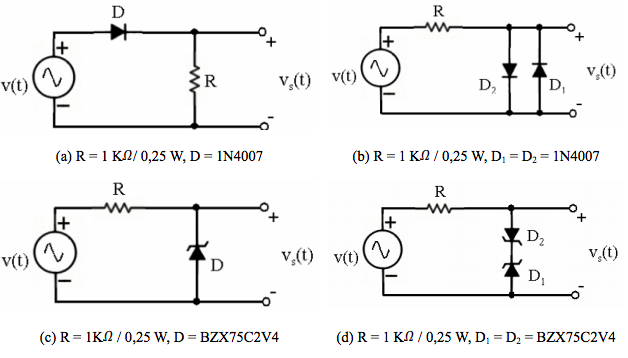
\includegraphics[width=.8\textwidth]{circuitos.png}
  \caption{Circuitos montados no procedimento experimental.}
  \label{fig:circuitos}
\end{figure}

\section{Experiência 1}

Para o circuito da figura \ref{fig:circuitos}(a) temos que a entrada ($v_I$) e saída ($v_o$) são definidas conforme a figura \ref{fig:io1} em que, no intervalo entre $x_0$ e $x_1$, o diodo $D$ encontra-se diretamente polarizado e, no intervalo $x_1$ a $x_2$, encontra-se reversamente polarizado, para esse circuito, não houve ruptura.

A característica de transferência $v_o \times v_I$ é caracterizada pela figura \ref{fig:diff1}.

\begin{figure}[h]
  \centering
  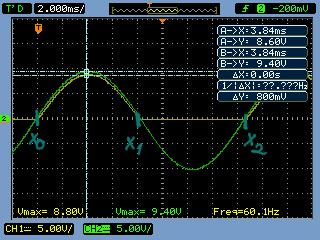
\includegraphics[width=.8\textwidth]{circuito-1a-esboco2.png}
  \caption{Gráfico da entrada (verde) e saída (amarelo) do circuito da figura \ref{fig:circuitos}(a).}
  \label{fig:io1}
\end{figure}

\begin{figure}[h]
  \centering
  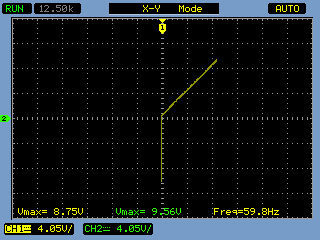
\includegraphics[width=.8\textwidth]{diferenca-1a.png}
  \caption{Gráfico da característica de transferência do circuito da figura \ref{fig:circuitos}(a) em que $v_o$ está no eixo horizontal e $v_I$ está no eixo vertical.}
  \label{fig:diff1}
\end{figure}

\section{Experiência 2}

Para o circuito da figura \ref{fig:circuitos}(b) temos que a entrada ($v_I$) e saída ($v_o$) são definidas conforme a figura \ref{fig:io2}  em que, no intervalo entre $x_0$ e $x_1$, o diodo $D_2$ encontra-se diretamente polarizado e $D_1$ encontra-se inversamente polarizado, no intervalo $x_1$ a $x_2$, $D_2$ encontra-se reversamente polarizado e $D_1$ encontra-se diretamente polarizado, para esse circuito, não houve ruptura.

A característica de transferência é caracterizada pela figura \ref{fig:diff2}.

\begin{figure}[h]
  \centering
  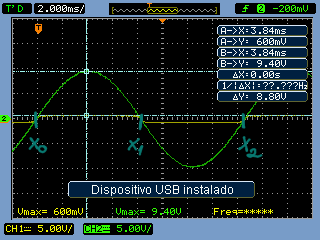
\includegraphics[width=.8\textwidth]{circuito-1b-esboco2.png}
  \caption{Gráfico da entrada (verde) e saída (amarelo) do circuito da figura \ref{fig:circuitos}(b).}
  \label{fig:io2}
\end{figure}

\begin{figure}[h]
  \centering
  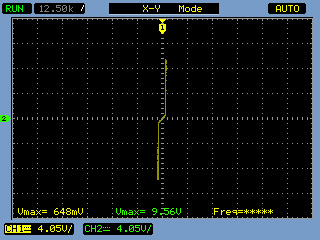
\includegraphics[width=.8\textwidth]{diferenca-1b.png}
  \caption{Gráfico da característica de transferência do circuito da figura \ref{fig:circuitos}(b) em que $v_o$ está no eixo horizontal e $v_I$ está no eixo vertical.}
  \label{fig:diff2}
\end{figure}

\section{Experiência 3}

Para o circuito da figura \ref{fig:circuitos}(c) temos que a entrada ($v_I$) e saída ($v_o$) são definidas conforme a figura \ref{fig:io3}  em que, no intervalo entre $x_0$ e $x_1$, o diodo $D$ encontra-se em ruptura, no intervalo $x_1$ a $x_2$, $D$ encontra-se diretamente polarizado, para esse circuito, houve polarização reversa em $D$ nos instantes $x_0$ e $x_2$.

A característica de transferência é caracterizada pela figura \ref{fig:diff3}.

\begin{figure}[h]
  \centering
  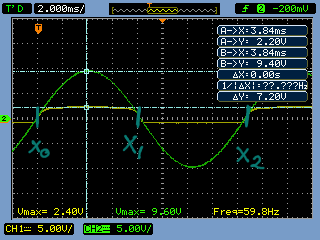
\includegraphics[width=.8\textwidth]{circuito-1c-esboco2.png}
  \caption{Gráfico da entrada (verde) e saída (amarelo) do circuito da figura \ref{fig:circuitos}(c).}
  \label{fig:io3}
\end{figure}

\begin{figure}[h]
  \centering
  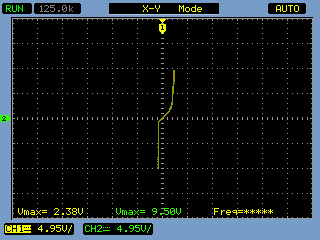
\includegraphics[width=.8\textwidth]{diferenca-1c.png}
  \caption{Gráfico da característica de transferência do circuito da figura \ref{fig:circuitos}(c) em que $v_o$ está no eixo horizontal e $v_I$ está no eixo vertical.}
  \label{fig:diff3}
\end{figure}

\section{Experiência 4}

Para o circuito da figura \ref{fig:circuitos}(d) temos que a entrada ($v_I$) e saída ($v_o$) são definidas conforme a figura \ref{fig:io4}  em que, no intervalo entre $x_0$ e $x_1$, o diodo $D_2$ encontra-se diretamente polarizado e $D_1$ encontra-se em ruptura, no intervalo $x_1$ a $x_2$, $D_2$ encontra-se em ruptura e $D_1$ encontra-se diretamente polarizado, para esse circuito, houve polarização inversa em $D_1$ nos momentos $x_0$ e $x_2$ e em $D_2$ no momento $x_1$.

A característica de transferência é caracterizada pela figura \ref{fig:diff4}.

\begin{figure}[h]
  \centering
  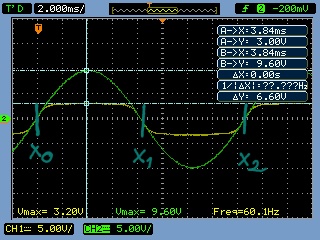
\includegraphics[width=.8\textwidth]{circuito-1d-esboco2.png}
  \caption{Gráfico da entrada (verde) e saída (amarelo) do circuito da figura \ref{fig:circuitos}(d).}
  \label{fig:io4}
\end{figure}

\begin{figure}[h]
  \centering
  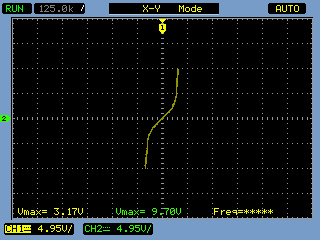
\includegraphics[width=.8\textwidth]{diferenca-1d.png}
  \caption{Gráfico da característica de transferência do circuito da figura \ref{fig:circuitos}(d) em que $v_o$ está no eixo horizontal e $v_I$ está no eixo vertical.}
  \label{fig:diff4}
\end{figure}

\chapter{Discussão}

\section{Comparação com o modelo ideal}
Para o circuito \ref{fig:circuitos}(a), um diodo ideal se comporta como um circuito aberto quando está inversamente polarizado, impedindo a passagem de corrente, zerando a saída. E o diodo se comporta como um curto circuito quando está diretamente polarizado,
permitindo, instantâneamente, que toda a corrente disponível passe pelo dispositivo, copiando a entrada na saída, assim como mostrado em vermelho na figura \ref{fig:comp1}.

\begin{figure}[h]
  \centering
  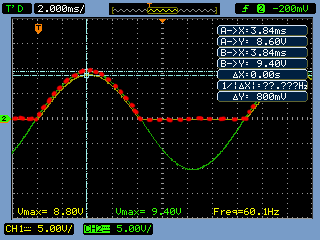
\includegraphics[scale = .7]{circuito-1a-esboco.png}
  \caption{Esboço do comportamento esperado para um diodo ideal para o circuito 1.}
  \label{fig:comp1}
\end{figure}
\pagebreak
O resultado obtido no experimento é muito similar ao do diodo ideal, com pequenas diferenças nos momentos em que o diodo está diretamente polarizado, visto que o diodo real tem um comportamento exponencial somado a uma queda de tensão no dispositivo.
Ao compararmos com o modelo de queda de tensão constante, podemos perceber que o comportamento é mais semelhante ao do diodo real, visto que considera a queda de tensão no dispositivo, mas com diferenças pois não considera o comportamento exponencial.

\\Para o circuito \ref{fig:circuitos}(b), considerando diodos ideais, não teríamos o comportamento limitante, mas sim a saída sempre em 0 V, visto que sempre haveria um curto circuito entre Vs e o nó de referêcia (relacionando com o modelo de queda de tensão constante, teríamos Vd = 0 V, limitando sempre em 0). Comportamento demonstrado em vermelho na figura \ref{fig:comp2}.

\begin{figure}[h]
  \centering
  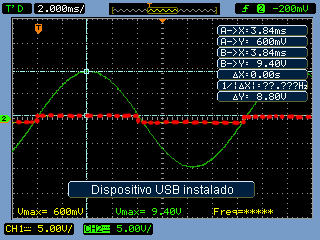
\includegraphics[scale = .7]{circuito-1b-esboco.png}
  \caption{Esboço do comportamento esperado para um diodo ideal.}
  \label{fig:comp2}
\end{figure}

\\Entretanto, considerando o modelo de queda de tensão constante, um dos diodos limitaria a tensão em 1,1 V instantâneamente no regime positivo da fonte de tensão quando diretamente polarizado e o outro diodo limitaria instantâneamente em -1,1 V no regime negativo da
fonte de tensão (quando este diodo estaria diretamente polarizado). Comportamento muito próximo do obtido experimentalmente, apenas não levando em consideração a curva exponencial durante a troca de regime da fonte de tensão e pequenas variações em Vd.

% \pagebreak

Para o circuito \ref{fig:circuitos}(c), se considerarmos o modelo de queda de tensão constante o modelo ideal de diodo zener, temos que quando o dispositivo está diretamente polarizado o circuito limita a saída em -Vd e quando está inversamente polarizado o circuito limata Vs em Vz. Assim como mostrado em vermelho na figura \ref{fig:comp3}.

\begin{figure}[h]
  \centering
  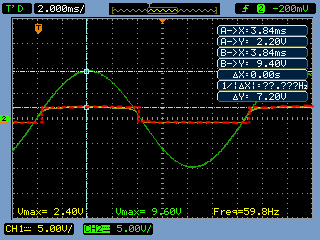
\includegraphics[scale = .7]{circuito-1c-esboco.png}
  \caption{Esboço do comportamento esperado para um diodo ideal.}
  \label{fig:comp3}
\end{figure}
\pagebreak
O comportamento do diodo real em relação ao ideal é muito similar, apenas não considerando a curva exponencial na troca de regime e pequenas variações em Vd e Vz.
Se o diodo Zener ideal possuísse um comportamento semelhar ao diodo ideal, teríamos apenas um curto circuito para qualquer regime da fonte de tensão.

\\Para o circuito \ref{fig:circuitos}(d), considerando o modelo de queda de tensão constante como o modelo ideal, temos o comportamento mostrado em vermelho na figura \ref{fig:comp4}.
Um dos diodos limita a tensão em Vz durante o regime positivo da fonte e o outro diodo limita em -Vz durante o regime negativo da fonte.

\begin{figure}[h]
  \centering
  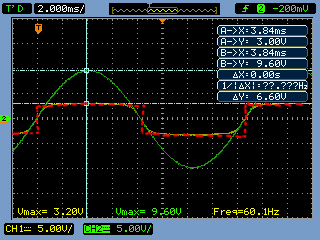
\includegraphics[scale = .7]{circuito-1d-esboco.png}
  \caption{Esboço do comportamento esperado para um diodo ideal.}
  \label{fig:comp4}
\end{figure}

O comportamento do diodo real em relação ao ideal é muito similar, apenas não considerando a curva exponencial na troca de regime e pequenas variações em Vz.
Se o diodo Zener ideal possuísse um comportamento semelhar ao diodo ideal, teríamos apenas um curto circuito para qualquer regime da fonte de tensão.

\section{Circuitos retificadores e limitadores}

O circuito retificador tem esse nome dado que para uma tensão menor que sua tensão de polarização direta ($V_d$), a saída torna-se uma tensão contínua, como podemos ver na figura \ref{fig:retificador}, no caso do circuito da figura \ref{fig:circuitos}(a) essa tensão de saída é 0.

O circuito limitador tem esse nome porque ele faz com que a tensão máxima que o circuito possa atingir seja seu $V_d$, como podemos ver na figura \ref{fig:limitador}.

\begin{figure}[h]
  \centering
  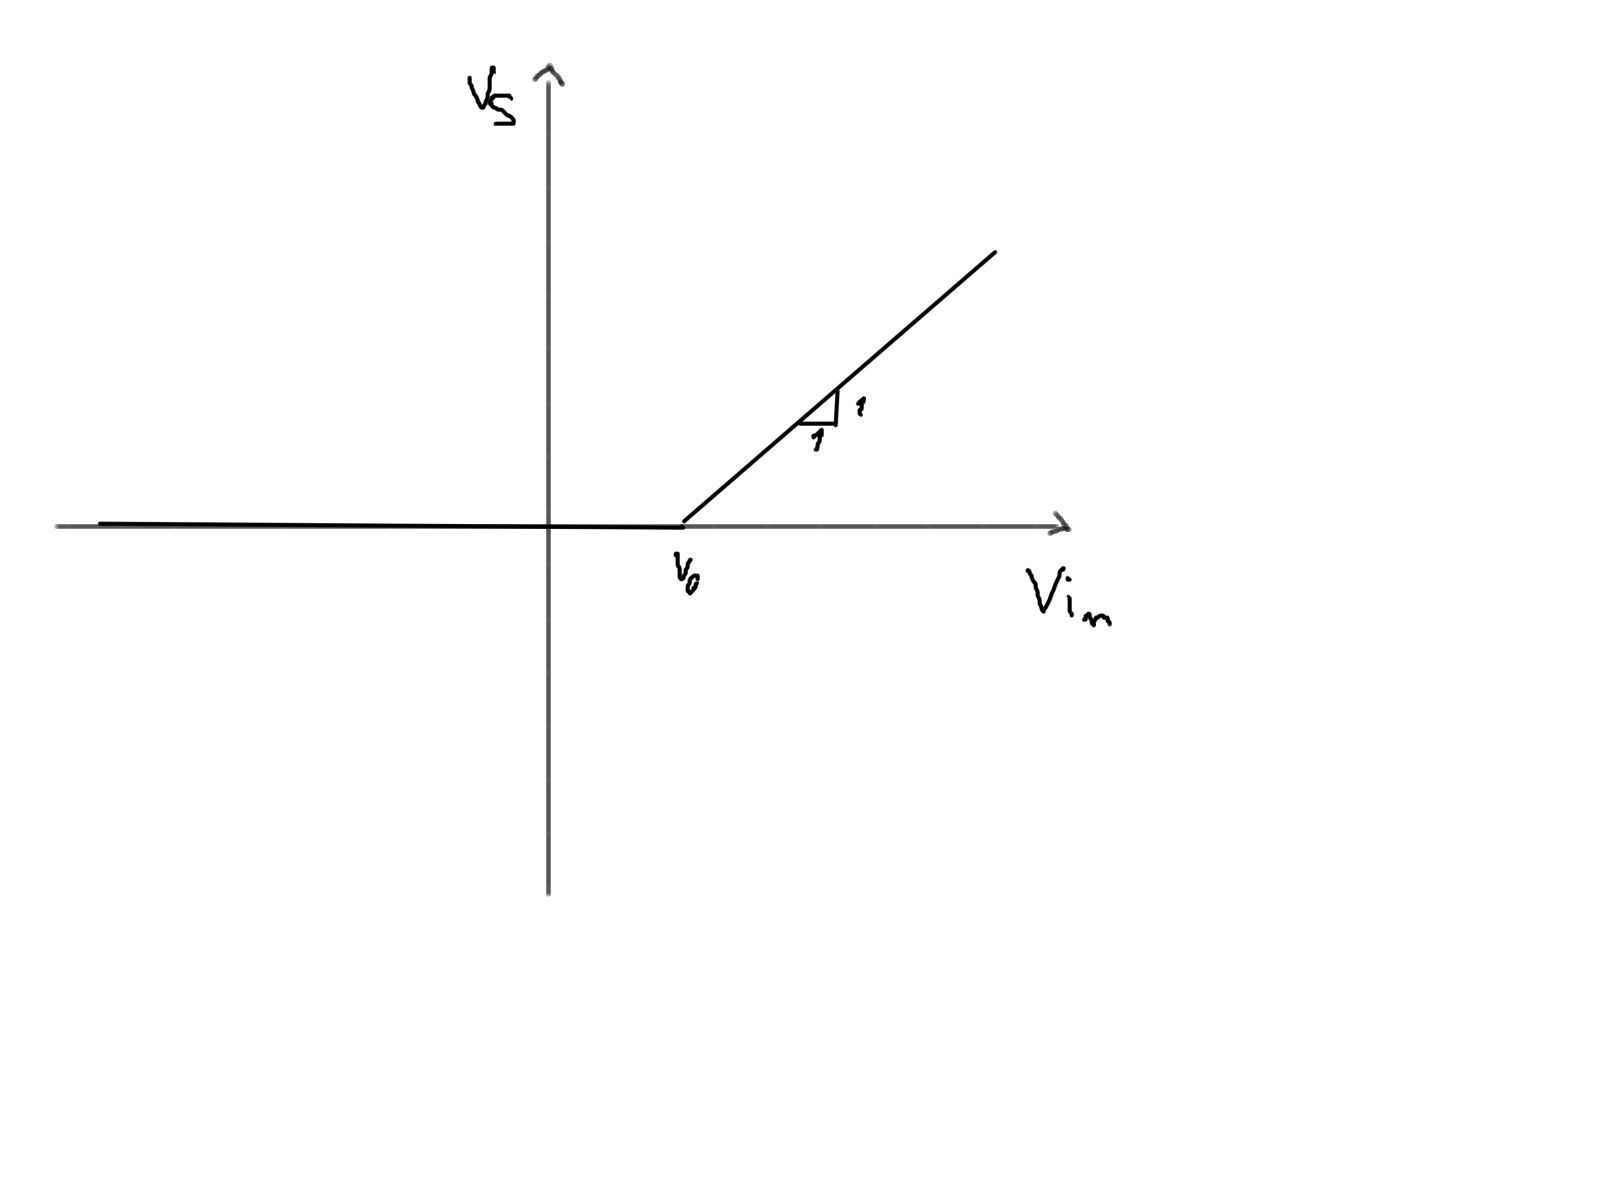
\includegraphics[width=.8\textwidth]{grafRetificador.jpeg}
  \caption{Gráfico da característica de transferência de um circuito retificador.}
  \label{fig:retificador}
\end{figure}

\begin{figure}[h]
  \centering
  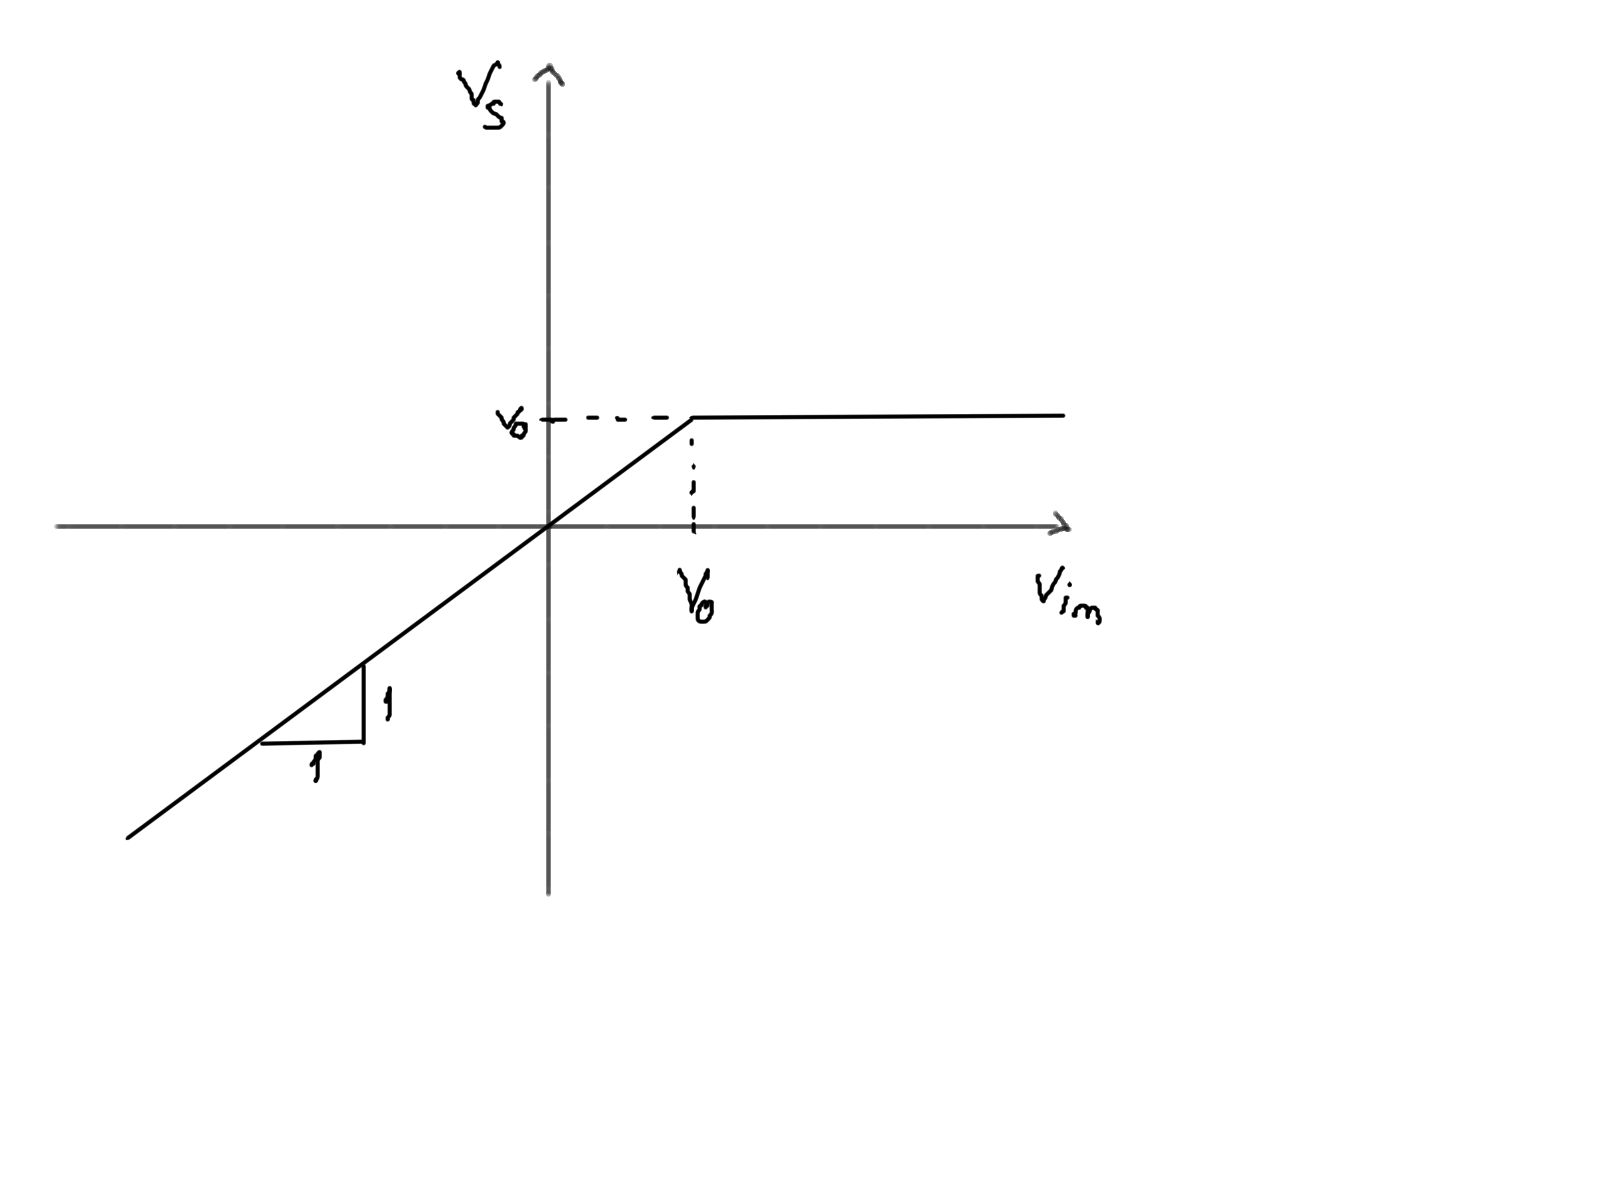
\includegraphics[width=.8\textwidth]{grafLimitador.jpg}
  \caption{Gráfico da característica de transferência de um circuito limitador.}
  \label{fig:limitador}
\end{figure}

Os circuitos da figura \ref{fig:circuitos} com exceção do circuito (a) podem ser considerados limitadores por reduzirem a amplitude da onda de saída ao valor da tensão de polarização direta ou de ruptura dos diodos do circuito.

\end{document}
